\chapter{IIR}
\label{chap:iir}

In this chapter the IIR filter is analyzed from its Matlab specification to the physical design.

\section{Matlab model}

We have updated \verb|my_iir_filter.m| to match the value of the given $N$ and $n_{b}$ values.
This script produces the filter's coefficients and saves the quantized filter's input in a file called \verb|samples.txt|, which is then used
by the C model (section \ref{sec:iir_c_model}) to test the goodness of the implementation.
The coefficients we have obtained are:

$$b_{0} = 423 \quad b_{1} = 846 \quad b_{2} = 423 \quad a_{0} = 1 \quad a_{1} = -757 \quad a_{2} = 401$$

After the C model's simulation, its results are read back to measure the {\it Total Harmonic Distortion}
($THD$). By keeping the internal representation on 12 bits we have measured $THD \approx -65.46\ dB$, which is
better than $THD_{target} = -30\ dB$, hence the whole filter has been implemented on 12 bits.


\section{C model}
\label{sec:iir_c_model}

In the C model we have only modified the coefficients to match the ones given by Matlab and the shift amount,
because a shift of \verb|NB-1| in our case resulted in an internal representation of 13 bits, while as said
earlier 12 bits were enough. Therefore, we have added a macro called \verb|INT_REPR| set to 1 which is
added to the previous term to obtain the target shift value. The output values have been stored in a file
called \verb|results_c_12bit.txt|.

\section{VHDL model}

\begin{figure}[!ht]
	\centering
	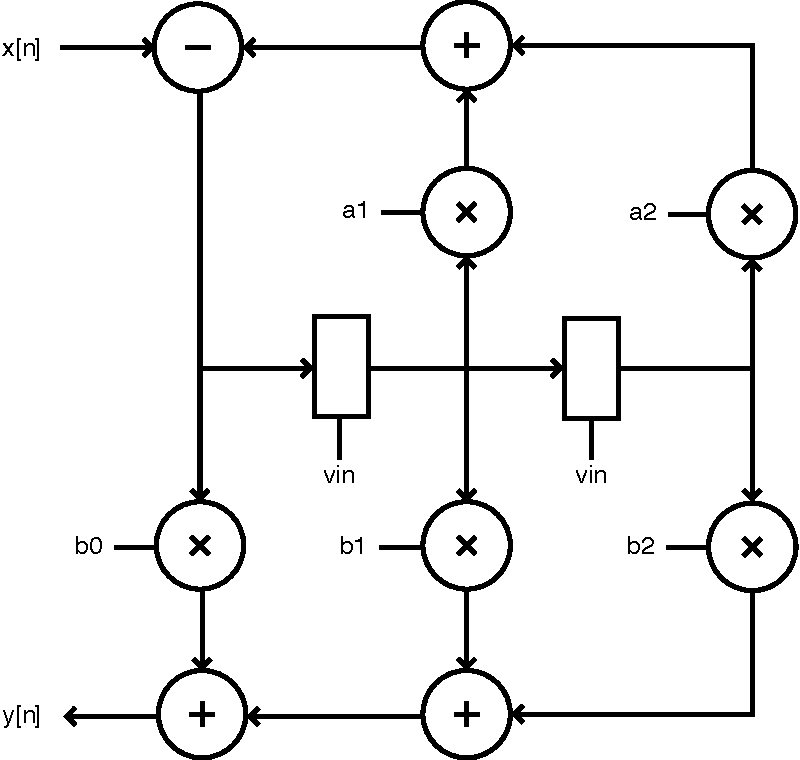
\includegraphics[width=0.4\linewidth]{./chapters/pictures/iir.pdf}
	\caption{IIR direct form II block diagram}
	\label{fig:iir}
\end{figure}

The filter has been implemented by deriving its structure from the C model and by using behavioral, generic components
for the arithmetic operations. The top module, instead, is not generic and its implemented in a structural way. It is
contained in the file \verb|iir.vhd|. In figure \ref{fig:iir} is shown the block diagram of the IIR.

The model entirely reflects the one described in C as it can be seen, the only peculiarity is in the organization of the
register's enable signals, not shown in picture \ref{fig:iir} (along with the input, coefficients and output registers)
to reduce the clutter.
Since the structure is so small no control unit has been developed. Instead, we have decided to add 1 bit registers to
store the delayed value of vin to correctly drive the filter.
The \verb|x[n]| register, along with the ones shown in the figure (that correspond to the C model's sw[i] array) and the
coefficients' registers are enabled by \verb|vin| itself. \verb|y[n]| register, on the other hand, takes as enable \verb|vin|
delayed by 1 clock cycle since it has to latch the value computed the cycle before. This means that the value of y[n] is
available to the filter's interface only the cycle after the register have been enabled, so the signal \verb|vout| corresponds
to \verb|vin| delayed by 2 clock cycles.

\subsection{Simulation}

This circuit has been simulated with {\it ModelSim}, that has written the simulation result in a file called
\verb|results_vhdl_12bit.txt|. The \verb|diff| tool has been run on the C model's output and this file to check that the
VHDL model was compliant with it.
To reproduce the simulation there is a script in the \verb|sim| folder called \verb|sim_script.tcl|.

\subsection{Logic synthesis}

The model described above has been synthesized with {\it Synopsys Design Compiler}. The synthesis has been run three times:

\begin{itemize}
    \item \textbf{Run 1}: to find the maximum clock frequency we have created a clock with period 0 with the command \verb|create_clock -name my_clk -period 0 clk|. With \verb|report_timing| we have found out that $t_{ck_{min}} = 2.81\ ns$.
    \item \textbf{Run 2}: to verify that $t_{ck_{min}}$ was actually a valid value we run a synthesis with a clock period $t_{ck} = t_{ck_{min}}$. The synthesis met the constraint and the area for this implementation is $A_{ck_{min}} \approx 4258\ \mu m^2$.
    \item \textbf{Run 3}: the synthesis with a clock period $t_{ck} = 4*t_{ck_{min}} = 11.24\ ns$ was executed. In this case the circuit is able to compute a value in $5.14\ ns$ with a slack of $5.99\ ns$, with an area $A \approx 3701\ \mu m^2$. 
\end{itemize}

To speed up the synthesis process two scripts are provided: \verb|setup.sh| and \verb|syn_script.tcl|. The former is used to create a clean synthesis environment,
the latter to run the synthesis. In this script is possible to choose among the settings of \textbf{Run 2}, by setting the variable \verb|use_tx4| to 0, and the settings
of \textbf{Run 3}, by setting \verb|use_tx4| to 1. 

\subsection{Power consumption estimation}

The resulting Verilog file produced in \textbf{Run 3} has been simulated again to check that the results were the same as the VHDL model and to obtain the circuit's switching activity.
The ModelSim script to calculate the switching activity is ???, that writes the file \verb|iir.sdf| in the \verb|netlist| folder.

This file, then, is read back in Synopsys by using the script \verb|syn_script_pwr.tcl| contained in the \verb|syn| folder. This script outputs \verb|report_switching_activity.txt|, a file containing the estimated power
consumption of the IIR based on the switching activity. Extracts of its content are reported below.

\begin{Verbatim}[fontsize=\small]
Cell Internal Power  = 278.3994 uW   (61%)
Net Switching Power  = 177.0917 uW   (39%)
                         ---------
Total Dynamic Power    = 455.4911 uW  (100%)

Cell Leakage Power     =  76.5232 uW


                 Internal         Switching           Leakage            Total
Power Group      Power            Power               Power              Power   (   %    )  Attrs
--------------------------------------------------------------------------------------------------
io_pad             0.0000            0.0000            0.0000            0.0000  (   0.00%)
memory             0.0000            0.0000            0.0000            0.0000  (   0.00%)
black_box          0.0000            0.0000            0.0000            0.0000  (   0.00%)
clock_network      0.0000            0.0000            0.0000            0.0000  (   0.00%)
register          83.7543           26.6556        9.8137e+03          120.2236  (  22.60%)
sequential         0.0000            0.0000            0.0000            0.0000  (   0.00%)
combinational    194.6452          150.4362        6.6709e+04          411.7907  (  77.40%)
--------------------------------------------------------------------------------------------------
Total            278.3995 uW       177.0918 uW     7.6523e+04 nW       532.0143 uW
\end{Verbatim}

\subsection{Place and route}

The Verilog file obtained in the previous step has been used to perform the {\it Place and route} on {\it Innovus}. We have rigorously followed all the steps
reported in the file \verb|documents.pdf| to complete this part, hence we will not repeat them here.

We have checked that 